\section{Future challenges}


\begin{frame}{Model physics}
  \begin{wideitemize}
    \item Uncertainties in parameterizations
    \item Gray zone of convection
  \end{wideitemize}
\end{frame}

\note{
  Uncertainties in parameterizations due to incomplete understanding of processes
  or representing impact of unresolved scales on the resolved scales.
  Statistical perturbations of model physics. Palmer 2001.

  Gray zone - historically, convection mostly unresolved.
  At 1 km, small-scale convective plumes still not resolved.
  Current global models assume convection is totally unresolved, not able to
  combine the impact of resolved and unresolved contributions to momentum and heat.
}

\begin{frame}{Model initialization}
  \begin{wideitemize}
    \item Lack of observations
  \end{wideitemize}
\end{frame}

\note{
  Only 5-10 percent satellite info used for forecast.
  Lack of wind information in the tropics - could be better with doppler-radar
  satellite data, not in use yet.
}

\begin{frame}{Computational challenges}
  \begin{figure}[htp]
    \centering
    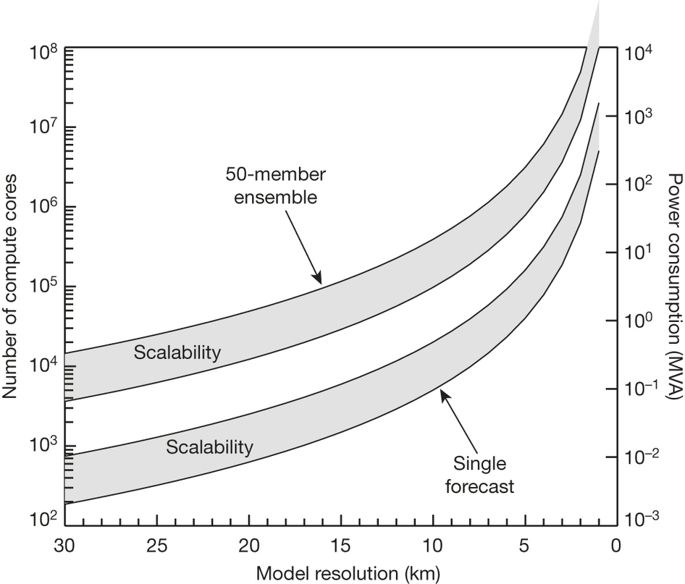
\includegraphics[width=0.6\textwidth]{figures/bauer_cpu.jpg}

  \parencite{bauer}
  \end{figure}
\end{frame}


\note{

Power usage - ECMWF affordable - 20 MVA.

1x1 km -> 100-1000 times as computationally intensive.
Expected to use 10 times more power.

Moores law is not expected to hold in the future -> Needs better scalability
(parallellization).

Storage capcaity - new hyper-spectral radiometers, thousands of channels ->
100 Gbyte per day.

}
